\documentclass[hyperref,french,usenames,xcolor=dvipsnames]{beamer}
\mode<presentation>
{
\usepackage{beamerthemesplit}
\usetheme{boxes}
%  \usecolortheme{orchid}
%       \setbeamercolor{alerted text}{fg=red!65!black}
  \setbeamercovered{transparent}
}
\usepackage{amsthm}
\usepackage{amsfonts}
\usepackage{amsmath}
\usepackage{graphicx}
%\usepackage{epsfig}
\usepackage{xspace}
\usepackage{stmaryrd}
%\usepackage{soul}
\usepackage[utf8]{inputenc}

\definecolor{newcolor}{rgb}{0, 0, .90}
\definecolor{impcolor}{rgb}{.90, 0, 0}
\definecolor{darkergreen}{rgb}{0,0.5,0}
\definecolor{myorange}{rgb}{0.8,0.7,0}
\definecolor{myviolet}{rgb}{0.7,0.0,0.7}

\definecolor{lightpurple}{rgb}{0.83,0.27,1}
\definecolor{lightblue}{rgb}{0.27,0.9,0.9}



%\newcommand{\texthl}[1]{{\color{blue}#1}}
%\newcommand{\jaune}[1]{{\color{blue}#1}}
%\newcommand{\texthlb}[1]{{\color{orange}#1}}
%\newcommand{\orange}[1]{{\color{orange}#1}}
%\newcommand{\verte}[1]{{\color{green}#1}}
%\newcommand{\trad}{{\color{orange}{\bf $\leadsto$}}}

%\newcommand{\textcite}[1]{{\color{lightpurple}[#1]}}
%\newcommand{\textciten}[1]{{\color{lightpurple}#1}}

\newcommand{\texthl}[1]{{\color{red}#1}}
\newcommand{\jaune}[1]{{\color{red}#1}}
\newcommand{\texthlb}[1]{{\color{orange}#1}}
\newcommand{\orange}[1]{{\color{orange}#1}}
\newcommand{\verte}[1]{{\color{green}#1}}
\newcommand{\trad}{{\color{orange}{\bf $\leadsto$}}}

\newcommand{\textcite}[1]{{\color{myviolet}[#1]}}
\newcommand{\textciten}[1]{{\color{myviolet}#1}}

\newcommand{\montilde}{$\sim$}


\title{Finding structure with randomness - Probabilistic Algorithms for Constructing Approximate Matrix Decomposition}

\author{Nelle \textsc{Varoquaux}}
\institute[ENS]{
\structure{
Ecole Normale Superieur de Cachan}
}

\date[09/12/11]{MVA - 14/12/11}

%\date[] % (optional)
%{}

\subject{Compressed Sensing - 14/12/11}

\AtBeginSection[] % Do nothing for \section*
{
  \frame<beamer>
  {
    \frametitle{Sommaire}
    \tableofcontents[current]
  }
}

\begin{document}

\frame{\maketitle}

\frame{
\frametitle{Problematic}

Traditional algorithms:
\begin{itemize}
\item QR
\item SVD
\item Eigenvalue/Eigenvector
\end{itemize}

are often:

\begin{itemize}
\item very expensive for large matrices
\item ill-adapted to matrices with missing or inacurrate data
\end{itemize}
}

\frame{

\begin{block}{Approximative Matrix Decomposition in Two stages}

\begin{itemize}
\item{Stage A}: Compute an orthornormal low rank basis $\bold{Q}$ such that, \\
  $\bold{A} \approx \bold{Q}\bold{Q}^T\bold{A}$

\item{Stage B}: Compute the matrix factorisation on $\bold{B} = \bold{Q}^T
\bold{A}$
\end{itemize}
\end{block}
}

\frame{
\begin{block}{The fixed precision problem}
Given $\bold{A}$ and $\epsilon$, find $\bold{Q}$ s.t.
$$\lVert \bold{A} - \bold{Q}\bold{Q}^T \bold{A} \lVert \leq \epsilon$$
\end{block}
\begin{block}{The fixed rank problem}
Given $\bold{A}$ and $k$, seek $\bold{B}$ s. t.
$$\lVert \bold{A} - \bold{Q}\bold{Q}^T \bold{A} \lVert \approx \min_{rank(\bold{B}) \leq
k} \lVert \bold{A} - \bold{B} \lVert$$
\end{block}
}

\frame{
\begin{block}{The proto-algorithm}

1. Draw an $n * (k + p)$ random matrix $\bold{\Omega}$ \\
2. Form the matrix $\bold{Y} = \bold{A} \bold{\Omega}$ \\
3. Construct a matrix $\bold{Q}$ whose columns form an othonormal basis for the
range of $\bold{Y}$ \\
\end{block}}

\frame{
\begin{block}{Stage A - Randomized Range Finder}
1. Draw an $n * l$ Gaussian random matrix $\bold{\Omega}$ \\
2. Form the $m * l$ matrix $\bold{Y} = \bold{A} \bold{\Omega}$ \\
3. Construct the $m * l$ matrix $\bold{Q}$ using the QR factorization
$\bold{Y} = \bold{QR}$
\end{block}
}

\frame{
\begin{block}{Stage A - Randomized Power Iteration}
1. Draw an $n * l$ Gaussian random matrix $\bold{\Omega}$ \\
2. For the $m * l$ matrix $\bold{Y} = (\bold{AA}^T)^q \bold{A} \bold{\Omega}$ via alternative
application of $\bold{A}$ and $\bold{A}^q$ \\
3. Construct the $m * l$ matrix $\bold{Q}$ using the QR factorization
$\bold{Y} = \bold{QR}$
\end{block}
}

\frame{
\begin{block}{Stage B - Direct SVD}
1. Form the matrix $\bold{B} = \bold{Q}^T \bold{A}$ \\
2. Compute the SVD of the matrix $ \bold{B} = \tilde{\bold{U}}\bold{\Sigma} \bold{V}^T$ \\
3. Form the orthonormal matrix $\bold{U} = \bold{Q} \tilde{\bold{U}}$ \\
\end{block}
}

\frame{
\begin{block}{Example 1 - Large Dense Matrix}
Matrix formed using the images of the \textbf{Olivetti} face dataset. \\
Goal: extract EigenFaces \\
Methods used: Randomized Power Iteration + Direct SVD
\end{block}

\begin{figure}[h]
\caption{Eigenfaces of the Olivetti Dataset}
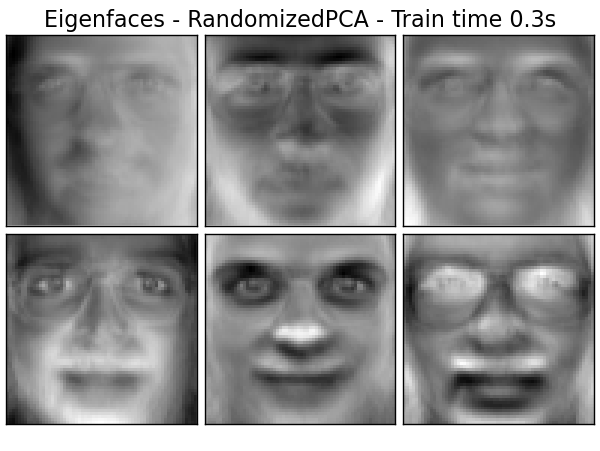
\includegraphics[width=200px]{./images/plot_faces_decomposition_2.png}
\end{figure}
}

\frame{
\begin{figure}
\caption{Power iteration with varying values of q}
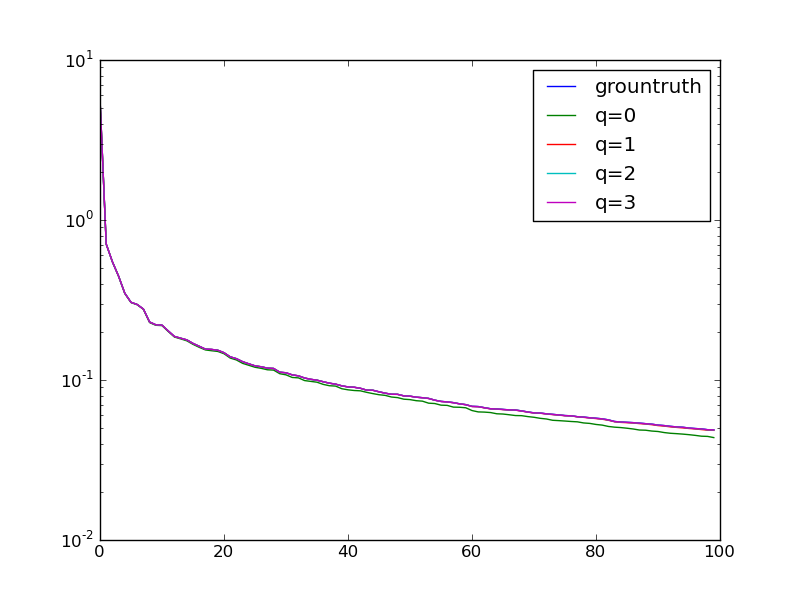
\includegraphics[width=300px]{./images/face_results.png}
\end{figure}
}

\frame{
\begin{center}
\huge{Conclusion}
\end{center}
}

\end{document}
